\section{Longstaff \& Schwartz pricing}
Another approach to American option pricing is manifest in the Least
Squares Monte Carlo algorithm (LSM), introduced in 2001 by Longstaff and
Schwartz \cite{longstaff2001valuing}. Here Monte Carlo
simulation is used to generate a corpus of possible price developments
of the underlying asset, and the option price is then calculated by
successively applying linear regression at each time step from
expiration to initiation time.

% In a historical context, Monte Carlo methods is relatively new
% approach to option pricing. Lattice methods where introduced in 1973,
% but only since 

\begin{algorithm}
  \begin{algorithmic}
    \Function{LSM}{$T$, $M$, $N$, $s_0$, $K$, $r$, $\sigma$}
    \State $\Delta t \gets \frac{T}{M}$
    \State $S \gets$ \Call{GeneratePricePaths}{$N$, $M$, $s_0$, $\sigma$, $\Delta t$, $r$}
    \State \Comment $N \times (M+1)$ matrix of $N$ paths
    \State $V_{M+1} \gets max(K-S_{M+1}, 0))$ \Comment Cash flow at expiry
    \For{$t \gets M-1$ \textbf{to} $1$}
    \State $E_t \gets max(K-S_t, 0)$ \Comment Exercise value
    \State $f_t \gets$ \Call{LeastSquares}{$\overline{S_t}$, $e^{-r\Delta t}\cdot\overline{V_t}$} % \Comment Find regression function $f_t$
    \State $\hat{C_t}$ $\gets$ $f_i(S_t)$ \Comment Expected value for continuation
    \State $V_t \gets $\textbf{if} $E_t > C_t > 0$ \textbf{then} $E_t$ \textbf{else} $e^{-r\Delta t}\cdot V_t$
 % max(F_t, E_t)$
    \EndFor
    \EndFunction
  \end{algorithmic}
  \vspace{2mm}
  \caption{Least Squares Monte Carlo algorithm for American put
    options. $\overline{S_t}$ and $\overline{V_t}$ selects those paths
    which are in the money, that is where $E_t > 0$.}
  \label{alg:lsm-algorithm}
\end{algorithm}

Algorithm \ref{alg:lsm-algorithm} presents the LSM algorithm.  The
approach is to first generate a large number of possible price
developments of the underlying, up till expiration. The algorithm
proceeds by moving backwards in time from expiration time, and at each
step estimating the value of continuation by least squares
regression. These estimates are then used to calculate the current
option price, before continuing to the next iteration.

We have left out how to generate price paths and perform the actual
least squares regression, these will be treated in more detail in the
subsequent sections.

\subsection{Path generation}
A standard approach to constructing the corpus of price paths is by
sampling paths of geometric Brownian motion.

This can be done by iterative application of the following equation:
$$S_{t+\Delta t}=S_te^{\Delta t(r-\sigma^2/2) + \sigma v\sqrt{\Delta t}}$$ where 
$v$ is a real number drawn from $\mathcal{N}(0,1)$, $\Delta t$ is the
size of the time period, and $\sigma$ is the volatility. Volatility is
the standard deviation of the option value over time and corresponds
in function to that of $u$ and $d$ in the binomial model. The
right-hand side consists of two parts where the first exponent
corresponds to the deterministic evolution of the price by the
riskless interest rate, and the second part corresponds to the
variation introduced from the Brownian motion. A derivation of the
equation can be found in the book \emph{Monte-Carlo Methods in
  Financial Engineering} by Paul Glasserman \cite[Section
3.2]{glasserman2003monte}.

\begin{algorithm}
  \begin{algorithmic}
    \Function{GeneratePricePaths}{$N$, $M$, $s_0$, $\sigma$, $\Delta t$, $r$}
    \State $S_0 \gets$ Initialize vector with $N$ repetitions of $s_0$
    \For{$i \gets 0$ \textbf{to} $M-1$}
      \State $V \gets$ Generate $N$ normally distributed random numbers
      \State $D \gets$ \textbf{parmap} $(\lambda v.\ e^{\Delta t(r-\sigma^2/2) + \sigma v\sqrt{\Delta t}})$ $V$
      \State $S_{i+1} \gets$ \textbf{parallelZipWith} $(+)$ $S_{i}$ $D$
    \EndFor
    \State \Return S
    \EndFunction
  \end{algorithmic}
  \caption{Brownian motion path generation}
  \label{alg:lsm-pathgeneration}
\end{algorithm}

% \todo{perhaps introduce Brownian Bridge alternative}

As long as we can generate independent random numbers in parallel this
generation can also be parallelized, as each path can be generated
independently.

\subsection{Random number generation}
A necessity for all applications of Monte Carlo methods is a source of
good random numbers. We cannot computationally generate ``true'' random
numbers, as they will always follow our chosen algorithm, but through
the use of \emph{pseudo-random number generators} (PRNGs) we can
generate sequences of numbers with approximately the same properties
as a completely random sequence. Such algorithms are widely used in both
Monte Carlo simulation and cryptography, but the choice of algorithm
depends on the application area as different PRNGs displays different
statistical properties.

An alternative scheme is that employed by a \emph{quasi-random number
  generator} (QRNG). Algorithms in this category aims for sequences
with low discrepancy, which is a measure of spacing in the
sequence. If we are to generate a sequence over some interval $[a,b]$,
discrepancy would be high if there were any subintervals $[c,d]$ with
proportionally few samples compared to other
intervals. Low discrepancy thus guarantees that proportionally equal
amounts of samples are made in all subintervals. We thus avoid gaps in
the sample space with few or no samples or conversely, regions with
high sample density. To illustrate, Figure \ref{fig:discrepancyplot}
shows a graph of a low-discrepancy sequence compared with sequence of
uniformly generated numbers from a PRNG.

\begin{figure}
	\centering
	\subbottom[]{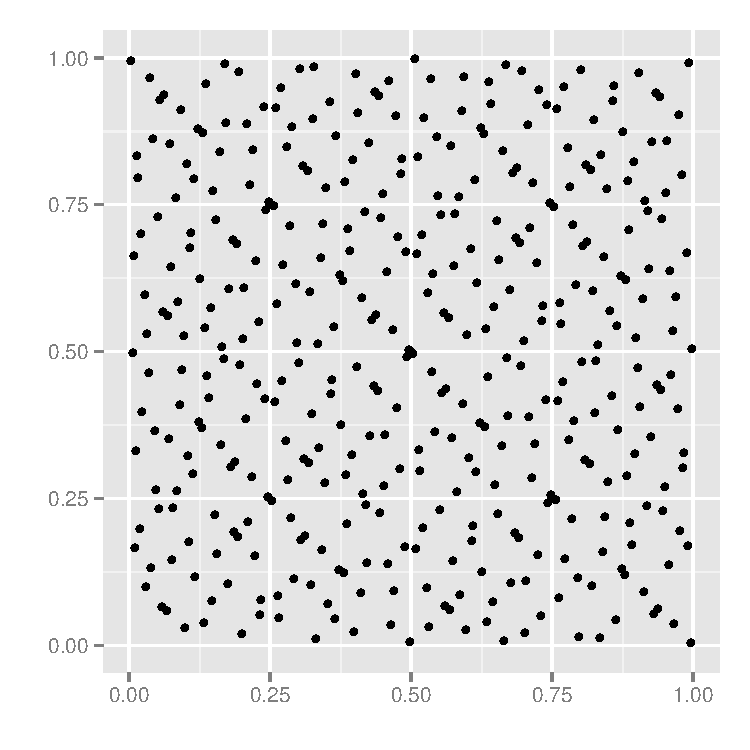
\includegraphics[width=0.45\textwidth]{graphics/2D-sobol-sequence.pdf}\hspace{0.55cm}\label{fig:2d-sobol-sequence}}
	\subbottom[]{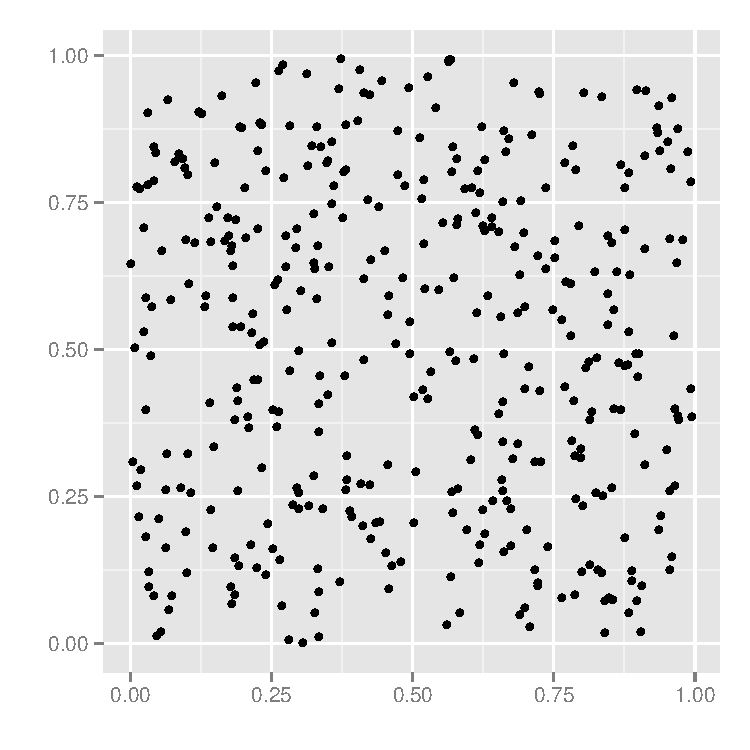
\includegraphics[width=0.45\textwidth]{graphics/2D-mersenne-sequence.pdf}\hspace{0.55cm}}

  \caption{\textbf{(a)} A 2D sequence of low-discrepancy numbers
    generated using the Sobol generator \textbf{(b)} A uniform 2D
    sequence of pseudorandom numbers generated with Mersenne twister
    PRNG}
\label{fig:discrepancyplot}
\end{figure}

QRNGs does not assure any other properties of random sequences and
does indeed follow rather visible patterns (see Figure
\ref{fig:2d-sobol-sequence}). It is not the aim to get close to
statistically random numbers, instead QRNG provides numbers suitable
for numerical integration, optimization and simulation. QRNGs have
several times been shown useful in financial Monte Carlo simulations
\cite{chaudhary2005american, couffignals2010quasi, dfine2009americanbasket}
%  \todo{perhaps mention the differences between their methods}
and a survey paper shows QRNGs beating PRNGs
when it comes to option pricing \cite{acworth1998comparison}. The
survey is 15 years old, so newer PRNGs might perform differently.
% \todo[noinline]{which other noteworthy?}

We will look closer at one particular low-discrepancy generator,
namely the Sobol sequence generator, by the Russian mathematician
I. M. Sobol \cite{sobol1967}. We chose the Sobol sequence because it
was the one used by an unrelated sample application from one of
HIPERFIT's industri partners. Also, the above mentioned survey
concludes that ``Sobol' points appear to give the best results among
the QMC sequences tested''.

\subsection{Sobol generator}
\label{sec:sobol}
We will not discuss why the numbers generated by the Sobol generator
maintain low discrepancy, but only focus on the algorithmic aspect of
computing the numbers.

Given a sequence of so called \emph{direction numbers}, $v_1, v_2,
\ldots$, the computation of Sobol-sequences is pretty straight forward:
$$x_i = b_1v_1 \oplus b_2v_2 \oplus \ldots \oplus b_lv_l$$
where $b_l\ldots b_3b_2b_1$ is the binary representation of $i$ in
$l$-bit representation. This simple algorithm is presented in Figure
\ref{alg:sobol-inductive}, where \textsc{ToBitVector} converts an
integer $i$ to its binary representation as an array of integers. In
our own implementations we have used $32$-bit integers. As computing
each number is independent of the other numbers, we can parallelise by
mapping \textsc{SobolInductive} over the indices.

The \textsc{SobolInductive} algorithm as well as the remaining
algorithms produces integer values in the range $[0, 2^l]$ and we thus
has to normalize this to $(0,1]$ to get a uniform distribution. In
addition, we have to convert this uniform distribution to a normal
distribution. This will be discussed in Section
\ref{sec:sampling_normaldist}.

\begin{algorithm}
  \begin{algorithmic}
    \Function{SobolInductive}{$v$,$i$}
    \State \Return \textbf{fold} $\oplus$ 0 (\textbf{zipWith} ($\times$) $v$ (\textsc{ToBitVector} $i$))
    \EndFunction
  \end{algorithmic}
  \caption{Generate element $i$ of the Sobol sequence using vector
    $v$ as direction numbers.}
  \label{alg:sobol-inductive}
\end{algorithm}

% \begin{algorithm}
%   \begin{algorithmic}
%     \Function{SobolInductive}{$v$,$n$}
%     \ParFor{$i \gets 0$ to $n-1$}
%     \State $A[i] \gets$ \textbf{fold} $\oplus$ 0 (\textbf{zipWith} ($\times$) (\textsc{ToBitVector} i) $v$)
%     \EndParFor
%     \EndFunction
%   \end{algorithmic}
%   \caption{Inductive Sobol generator.}
%   \label{alg:sobol-inductive}
% \end{algorithm}

If one seeks for a sequential algorithm for Sobol sequence generation,
we can improve on the above by using the Gray code binary
representation of the index instead of the ordinary, whereby a
recursive definition of Sobol sequences can be made
\cite{bratley1988algorithm}. It has been shown that
\begin{equation}
x_{i+1} = x_i \oplus v_c\label{eq:sobol-recurse}
\end{equation}

where $c = \mathit{lsb}(i)$ is the index of the least set bit in
$i$. A sequential algorithm using this strategy is presented in Figure
\ref{alg:sobol-recursive}.

\begin{algorithm}
  \begin{algorithmic}
    \Function{SobolRecursive}{$v$,$A$,$i$,$n$}
    \State $x_i \gets$ \textsc{SobolInductive}($v$, \textsc{GrayCode} $i$)
    \State $end \gets i + n$
    \While{$i < end$}
    \State $c \gets \mathrm{lsb}(i)$
    \State $x_ {i+1} \gets x_i \oplus v_c$
    \State $i \gets i + 1$
    \EndWhile
    \EndFunction
  \end{algorithmic}
  \caption{Sequentially generate elements $i$ through $i+n-1$ of the
    Sobol sequence and store results at the appropriate indices of
    the $x$ vector.}
  \label{alg:sobol-recursive}
\end{algorithm}

This approach does not output the same sequence though, but it has
been shown \cite{bratley1988algorithm} that Gray code based sequences
also displays the property of low discrepancy, as it is merely a
scrambling (reordering) of prefixes of the original Sobol
sequence. Conversion to Gray code representation can be done through
single shift and an exclusive-or operation, which makes for a cheap
sequential algorithm.

The two approaches can be combined to achieve an alternative parallel
implementation. The sequence that needs to be generated is divided in
chunks onto each processing element, the inductive algorithm is used
to initialize each of the chunks and the recursive algorithm is then
used to fill out the space. The algorithm is shown in Figure
\ref{alg:sobol-parallel-1}

\begin{algorithm}
  \begin{algorithmic}
    \Function{SobolParRecurse}{$v$,$n$}
    \State $x \gets$ allocate vector of length $n$
    \State $m \gets$ number of processor cores (e.g. CUDA cores)
    \State $r \gets \lceil n/m \rceil$
    \ParFor{$p \gets 0$ to $m-1$}
    \State $start \gets p\cdot r$
    \State \textsc{SobolRecursive}($v$,$x$,$start$,$\min(r,n-start)$)
    \EndParFor
    \EndFunction
  \end{algorithmic}
  \caption{Parallel Sobol sequence generator.}
  \label{alg:sobol-parallel-1}
\end{algorithm}

The problem with this algorithm is that its memory behavior is not
suitable for GPUs. Programs that does not coalesce memory accesses,
such that all cores act on the same block simultaneously, incurs a big
performance penalty. With this algorithm, each thread will write very
dispersed, as each thread will fill out each its own region of the
array A.

Luckily, an alternative strategy has been shown by Thomas Bradley et
al. \cite[Chapter~16]{hwy2011emerald}. They observed that applying
\eqref{eq:sobol-recurse} several times, would lead to repeated
exclusive or operations with the same direction number. As the
\emph{exclusive or} operation is associative, commutative and is its
own inverse, some of these operations will cancel out. Especially,
when skipping a power of two ahead, all but two exclusive or
operations will cancel out. The least set bit will change in a
systematic way, and analysis shows that (see the above mentioned book
chapter):

\begin{equation}
  \label{eq:sobol-skipahead}
  x_{i+2^p} = x_i \oplus v_p \oplus v_{q(i)}
\end{equation}

where $q(i) = lsb(i \blor (2^p - 1))$. We use $\blor$ for bitwise or.

This fact can be used to develop a parallel algorithm which is memory
efficient on GPU architectures. Instead of each letting each thread
fill a separate block of memory using \eqref{eq:sobol-recurse}, we can
instead let all threads cooperate on filling one block at a time, by
using the inductive algorithm (Algorithm \ref{alg:sobol-inductive}) to
fill the first block of memory and use \eqref{eq:sobol-skipahead} to
fill each successive block. This thus requires a skipsize of a power
of two.

On a GPU this can done by letting a group of $2^b$ blocks of size
$2^p$ threads cooperate on filling a block of size $2^{p+b}$ before
continuing work on the next block.

This also illustrates that optimized GPU algorithms in some cases
needs to instruct kernel scheduling should be, as we need to make sure
that the size of a block and the number of blocks is a power of two,
and the algorithm needs information about these parameters.

\todo{The survey should be aware of this: How much control do we have
  over kernel execution in Nikola and Accelerate? Is it possible to
  drop down to a lower layer (without writing CUDA C) for such
  implementations?}


% \begin{align}
%   x_{n+4} & = x_n \oplus v_{lsb(n)} \oplus v_{lsb(n+1)} \oplus v_{lsb(n+2)} \oplus v_{lsb(n+3)} \\
%          & = x_n \oplus v_1 \oplus v_1 \oplus v_2 \oplus v_3 \\
%          & = x_n \oplus v_2 \oplus v_3 \\
% \end{align}

\begin{algorithm}
  \begin{algorithmic}
    \Function{SobolSkipping}{$v$, $n$, $p$, $b$}
%    \State $p \gets$ number of processor cores (e.g. CUDA cores)
%    \State $r \gets \lfloor n/m \rfloor$
    \ParFor{$i \gets 0$ \textbf{to} $2^{p+b}-1$}
    \State $x_i \gets$ \textsc{SobolInductive}($v$, \textsc{GrayCode} $i$)
    \While{$i < n$}
    \State $q \gets lsb(i \blor (2^{p+b} - 1))$
    \State $x_{i+2^{p+b}} \gets x_i \oplus v_{p+b}~\oplus v_q$
    \State $i <- i+2^{p+b}$
    \EndWhile
    \EndParFor
    \EndFunction
  \end{algorithmic}
  \caption{Parallel Sobol sequence generator. $v$ is the direction
    vector, $n$ is the length of the sequence, $2^p$ is the block size
    and $2^b$ is the number of blocks.}
  \label{alg:sobol-parallel-2}
\end{algorithm}

In the same book chapter they present skip-ahead strategies for two
PRNGs, the Mersenne Twister (the MT19937 variant) and L'Ecuyer's
Multiple Recursive Generator (MRG32k3a). \todo{Write some more about
  how they parallelise}

\subsection{Sampling the standard normal distribution}
\label{sec:sampling_normaldist}
The Sobol sequence generator as well as most other PRNGs and QRNGs
draws samples uniformly from the interval $(0,1]$ ($0$ is not
included, as we often want to avoid negative samples). In our
application we need samples from the standard normal distribution,
$\mathcal{N}(0,1)$, and thus a transformation is necessary.

The standard approach to convert from a uniform distribution to any
other distribution is by inversion of the cumulative distribution
function (CDF). It not possible to compute the inverted CDF exactly
for the normal distribution, but approximations exists. The algorithm
that seems the most popular when we have to do with QRNGs is called
the ``Beasley-Springer-Moro'' algorithm or ``Moro's inversion''. This
algorithm uses a result by Beasley and Springer from
\cite{beasley1977algorithm} to approximates the inverse CDF of the
standard normal distribution by
$$norminv_1(u) = \frac{\sum^3_{n=0}a_n(u-1/2)^{2n+1}}{1+\sum^3_{n=0}b_n(u-1/2)^{2n}}$$
on the interval $u \in [0.5, 0.92]$ for a specific set of constants
$a_n$ and $b_n$, see \cite[page 67-68]{glasserman2003monte}. Boris
Moro found \cite{moro1995full} that he could approximate the remaining
interval $u \in (0.92, 1]$ by $$norminv_2(u)= \sum^8_{n=0}c_n
log^n(-log(1-u))$$ where $c_n$ are additional constants, also given in
\cite{glasserman2003monte}. With this, the inverse CDF of the standard
normal distribution can now be written as:
$$cdf^{-1}(u) = \left\{
\begin{array}{ll}
  norminv_1(u) & \mathrm{if}~ 0.5 \leq u \leq 0.92\\
  norminv_2(u) & \mathrm{if}~ 0.92 < u < 1\\
  - cdf^{-1}(1-u) & \mathrm{if}~0 < u < 0.5\\
\end{array}\right.$$

\subsection{Least Squares solvers}
The only remaining element of the Longstaff \& Schwartz algorithm that
we need to discuss is the least squares regression. What we need is a
way of smoothing out the variation in the paths, by representing their
change from one point in time to the next by a function. We have a set
of stock prices $S_t$ and a set of option values $V_t$ and wants to
find the polynomial $f$ of a degree $d$ that is as close to these
coordinates as possible. That is, we want the coefficients
$\mathbf{x}$ for the polynomial that minimizes the error:

$$min_\mathbf{x} \sum^{N}_{i=0}(V_{t,i}-f(S_{t,i},\mathbf{x}))^2$$

to generalize this, we will use $a$ and $b$ in the rest of this
section, such that:
$$min_\mathbf{x} \sum^{N}_{i=0}(b_i-f(a_i,\mathbf{x}))^2$$

In our case, $f$ will take the shape of a polynomial:
$$f(\mathbf{a},\mathbf{x}) = x_1 + x_2a_i + x_3a_i^2 \ldots x_da_i^{d-1}$$
and this gives rise to a linear system of equations. Each equation
originating from a coordinate $(a_i, b_i)$. We write the system as:

\begin{equation}
  \label{eq:vandermonde}
  \mathbf{Ax} =
  \left(
  \begin{array}{ccccc}
    1 & a_1 & a_1^2 & \ldots & a_1^{d-1} \\
    1 & a_2 & a_2^2 & \ldots & a_2^{d-1} \\
     & & \vdots & & \\
    1 & a_n & a_n^2 & \ldots & a_n^{d-1} \\
  \end{array}\right)
  \left(
  \begin{array}{c}
     x_1 \\
     x_2 \\
    \vdots \\
     x_n \\
  \end{array}\right)
=
  \left(
  \begin{array}{c}
     b_1 \\
     b_2 \\
    \vdots \\
     b_n \\
  \end{array}\right)
= \mathbf{b}
\end{equation}

The $\mathbf{A}$ matrix is called a Vandermonde matrix.  To find the
minimizing $x$ vector, we want to minimize the residual vector
$\mathbf{r} = \mathbf{b} - \mathbf{Ax}$. By \todo{magic} we know that
we can find the minimizing $\mathbf{x}$ by solving the system
$\mathbf{A}^T\mathbf{A}\mathbf{x} = \mathbf{A}^T\mathbf{b}$.

There are several ways to solve such systems, for instance
LU-decomposition, QR-decomposition or Cholesky-decomposition. We have
chosen to implement Cholesky-decomposition, though that choice was a
bit arbitrary.

With Cholesky decomposition we find a lower triangular matrix
$\mathbf{L}$ such that $\mathbf{A} = \mathbf{LL}^T$. And now forward
and then backward substitution can be used to find the minimizing
$\mathbf{x}$.

%%% Local Variables:
%%% mode: latex
%%% TeX-master: "../master"
%%% End:
